\documentclass[10pt,conference]{IEEEtran}
\usepackage[utf8]{inputenc}
\usepackage{amsfonts,amsmath,amssymb,amsthm,amstext,latexsym}
\usepackage{subfig}
%\usepackage{mathdots}
\usepackage{url}
\usepackage{multirow}
\usepackage{tikz}
\usepackage{todonotes}
\usetikzlibrary{calc}
\usetikzlibrary{arrows,shapes}
\usetikzlibrary{patterns,decorations}
\newtheorem{theorem}{Theorem}
%opening

\pagestyle{plain}

\title{Approximating a Multi-Grid Solver}

\author{

    \IEEEauthorblockN{Valentin Le F\`{e}vre}
    \IEEEauthorblockA{
        %Barcelona Supercomputing Center\\i
        %Spain\\
        \'{E}cole Normale Supérieure de Lyon\\
        %France\\
        valentin.le-fevre@ens-lyon.fr}
    \and
    \IEEEauthorblockN{Leonardo Bautista-Gomez}
    \IEEEauthorblockA{
        Barcelona Supercomputing Center (BSC)\\
        %Spain\\
        leonardo.bautista@bsc.es}
    \and
    \IEEEauthorblockN{Marc Casas}
    \IEEEauthorblockA{
        Barcelona Supercomputing Center (BSC)\\
        %Spain\\
        marc.casas@bsc.es}
}

\begin{document}

\maketitle
\begin{abstract}
    This paper studies trade-offs between accuracy and execution time in a
    multi-grid solver: BoomerAMG. Since a linear system solver is never really
    exact, it is actually relevant to investigate whether it is possible to
    save time and energy by reducing precision during some steps while keeping
    results within the targeted accuracy . We first introduce a different cycle
    shape than the classic V-cycle used in multi-grid solvers. We show that it
    provides a usually faster convergence rate by running some tests on a
    distributed system with large input problems. Then, we propose a dynamic
    bit-width changing algorithm that is able to adapt the execution time of
    floating-point operations according to the accuracy needed. In particular,
    we are able to reach the same results as a double-precision floating point
    algorithm while gaining 15\% improvement of the execution time on a GPU.
\end{abstract}

\section{Introduction}
\label{sec:intro}

\section{Introduction}
\label{sec:intro}

Multi-Grid (MG) solvers are a class of linear methods~\cite{Hackbusch1991} that
emerged in the 80's to increase the convergence rate of more classical
iterative methods.  They became even more important with the advent of very
complex scientific applications~\cite{Ashby1996}, which required very powerful
linear solvers.  The usage of MG solvers has become a common practice in
today's parallel systems due to the good scalability properties this methods
display, which have been detailedly analyzed and modeled~\cite{Gahvari11}.
Also, MG solvers have been reported to display more robustness against silent
data corruptions than traditional iterative methods deployed over a single
grid~\cite{Casas12}, which also implies they behave well under reduced accuracy
scenarios.

Multi-Grid\ldo{Are we going to use MG or Multi-Grid? We should be consistent}
algorithms rely on a grid of evaluation points that discretize the
domain of a continuous differential equation.  Typically, MG schemes are
defined by coarsening a fine-grain grid until reaching a small set of
evaluation points where a direct method can be applied.
%This grid is represented using different granularity levels that are used to
%determine a solution on the inaccurate and coarse grids.
Solutions obtained on the inaccurate and coarse grids are used on the more
accurate and fine-grain levels to accelerate the process of obtaining the final
solution of the system.
%For example, if we want to solve an equation of the form: \[ -u^{''}(x)+au(x)
%= f(x),\quad 0<x<1, \quad u(0)=u(1)=0, \] where $a$ is some constant, $f$ a
%function and $u$ an unknown function, we can transform it into a discrete
%problem by selecting $N$ evaluation points $x_1,\dots,x_N$ and using taylor
%expansion to express the second derivative term $u^{''}(x_i)$ as a weighted
%sum of $u(x_j)$ for some values of $j$.  Then to define coarser grids, a
%simple way to do it is to divide the number of evaluation points and transform
%the original equation into another discrete problem (thus using evaluation
%points $x_1,x_3,\dots,x_N$).  Typically, multi-grid schemes are defined by
%coarsening a fine-grain grid until reaching a small enough set of evaluation
%points on which a direct solve would be fast.
Multi-grid solvers typically consist of three phases: The \textit{Relaxation},
\textit{Restriction} and \textit{Interpolation} phases.  The relaxation phase
applies a few steps of an iterative solver like Jacobi or Gauss-Seidel at a
certain coarseness level.  The restriction phase propagates the algorithmic
state to a coarser grid by means of linear transformations while the
interpolation phase maps the coarser estimate to the finer version and adjusts
the current solution with the new error.

One common way of orchestrating a Multi-Grid Solver execution is via a V-cycle,
where we first iterate on the finest grid, then the second finest grid and so
on until reaching the coarsest grid where a direct solve is used instead of an
iterative method as the problem size has become smaller.  Then we iterate again
on all the other grids in the reverse order to have a solution expressed with
the initial fineness of the grid.  Different parameters, such as the iterative
method used at each step or the fineness of the grid and the previously
mentioned cycle shape, affect the convergence rate of the algorithm.

%Typically, multi-grid schemes are defined by coarsening a fine-grain grid
%until reaching a small enough set of evaluation points on which a direct solve
%would be fast.  Multi-grid solvers then perform several steps of an iterative
%method like Jacobi~\cite{} or Gauss-Seidel~\cite{} switching between the
%different grids by interpolating or restricting the solution of the previous
%step.  More precisely, a multi-grid algorithm has a parameter which is the
%cycle shape.  The cycle shape determines in which order and on which
%coarsening of the grid an iterative method is used. The classical cycle shape
%is the V-cycle where we first iterate on the finest grid, then the second
%finest grid and so on until reaching the coarsest grid where a direct solve is
%used instead of an iterative method as the problem size has become smaller.
%Then we iterate again on all the other grids in the reverse order to have a
%solution expressed with the initial fineness of the grid.  Different
%parameters, such as the iterative method used at each step or the fineness of
%the grid and the previously mentioned cycle shape, affect the convergence rate
%of the algorithm. For example, using a grid with only a few evaluation points
%decreases the execution time but deteriorates the accuracy of the final
%result. In the other way, it is possible to increase the quality of the result
%by using a finer grid but at the cost of a performance degradation.

In this context, this paper investigates different trade-offs between accuracy
and execution time for MG algorithms. This paper focuses its effort on
one of the most popular parallel implementation of a multi-grid solver, the
BoomerAMG~\cite{boomerAMG}, implemented in the HYPRE
library~\cite{Falgout2002}.  This paper makes the following contributions
beyond the state-of-the-art:

\begin{itemize}

    \item We evaluate the impact of parameters of the solver such as the shape
        of cycles and the number of iterations.

    \item We propose a cycle configuration and show that it is equally or more
        efficient than the original algorithm.

    \item We \leo{evaluate the impact of different floating-point precisions on
        the time to completion while reaching full accuracy on the final
        result.}

    \item We propose an algorithm that dynamically adapts the precision of the
        MG algorithm variables to increase performance and efficiency.

    \item We \leo{perform a large evaluation and demonstrate the we can reduce by
        15\% the execution time needed to reach the same quality result as the
        original double-precision algorithm and up to 30\% for smaller
        accuracies.}

\end{itemize}


\leo{The reminder of this paper is organized as follows:
Section~\ref{sec:motivation} introduces the motivations for this work.
Section~\ref{sec:pruning} investigates the impact of different parameters on
the time to completion.  Section~\ref{sec:precision} explores
precision-performance trade-offs.  Section~\ref{sec:related} discuss other
related works and Section~\ref{sec:conclusions} concludes this paper.}



% \section{The multi-grid algorithm}
%
%\section{Multi-Grid Algorithm}
\label{sec:algo}

\leo{A very brief introduction to the MG algorithm.. }

%\subsection{Definitions}

%\begin{itemize}
% \item A system of equations is represented by the following equation: $Ax=b$, where $A \in \mathcal{M}(\mathbb{R})^{n\times n}$ and $b \in \mathcal{\mathbb{R}}^n$ are given and
% $x \in \mathbb{R}^n$ is the unknown. The \emph{exact} solution of this system will be denoted by $\widetilde{x}$.
% \item A level is an integer between $1$ and $L$. Level $1$ will be called the finest level, and level $L$ will be called the coarsest level.
%  \item The restriction of $A$ (or $b$ or $x$) to level $l$ will be denoted by $A^l$ (or $b^l$ or $x^l$). We have $A^1 = A$ (and $b^1=b,x^1=x$).
%  \item We define a set of $L-1$ restriction matrices $R_1,\dots,R_{L-1}$ such that $R_l b^l = b^{l+1}$. We also define some prolongation matrices $P_1,\dots,P_{L-1}$ such that $P_{l}b^{l+1} = b^l$.
%  In other words, we have $P_l = {R_l}^{-1}$ (left inverse) and we build the $A^l$ matrices as follows: $A^{l+1} = R_l A^l P_l$.
%  \item We denote by $e^l$ the error at level $l$, that is the vector such that $x^l + e^l = \widetilde{x^l}$, that is to say $\widetilde{x^l}-x^l$.
%  We also define the residual at level $l$, $r^l = b^l - A^lx^l$. As $b^l = A^l\widetilde{x^l}$, we can also write $r^l = A^le^l$.
%  \item We derive the relative residual norm at any step $i$ in the algorithm
%  by the norm of the residual at this step, $||b^l - A^lx^l_i||$, divided by the norm of the initial residual, $|| b^l - A^lx^l_0||$.\\ We also define the notion of \emph{tolerance}
%  as an real value between 0 and 1, which is a threshold for stopping an algorithm. In multi-grid algorithms, this threshold will be on the residual norm.
%  \item We call relaxation a step of an iterative method for solving linear systems (such as Jacobi, Gauss-Sneidel, \dots). Formally, for a vector $x \in \mathbb{R}^n$, it represents the computation of
%  $x \leftarrow Mx + c$ where $M \in \mathcal{M}(\mathbb{R})^{n\times n}$ and $c \in \mathcal{\mathbb{R}}^n$ are defined depending on the method used.
% \end{itemize}

%\subsection{The V-cycle}
%
%  The goal of the algorithm is to improve the efficiency of iterative methods. Indeed, the choice of the starting vector $x$ on which to apply relaxations has consequences on the convergence
%  time of the solver, and depending on the system to solve, the factor of convergence (related to the matrix $M$) can be close to 1.\\
%  Here the idea is to do some relaxations and then correct the value of $x$ by adding to it the corresponding error term. However, this error term cannot be computed easily (otherwise,
%  solving the problem would be done by computing the error term and adding it to $x$). Multi-grid solvers instead use recursion to compute the error term. The stopping parameter for the
%  recursion will be determined by decreasing the sizes of vectors and matrices (thus loosing some accuracy but saving time).
%  Formally, we can sum up the algorithm as follows:
%
%  MG$(l,x,f,\alpha_1,\alpha_2)$:
%  \begin{itemize}
%    \item If $l = L$, return $x = {A^L}^{-1} f$ (exact solve);
%    \item Else:
%    \begin{enumerate}
%      \item Relax $x$ $\alpha_1$ times using an iterative method (matrix $A^l$, right hand side $f$);
%      \item $r \leftarrow R_l ( f - Ax )$;
%      \item $y \leftarrow 0$:
%      \item MG$(l+1,y,r,\alpha_1,\alpha_2)$;
%      \item $e \leftarrow P_{l} y$;
%      \item $x \leftarrow x+e$;
%      \item Relax $x$ $\alpha_2$ times using an iterative method (matrix $A^l$, right hand side $f$);
%   \end{enumerate}
%  \end{itemize}
%  The algorithm is then executed by setting $x^l \leftarrow 0$ and then executing MG$(1,x^l,b^l,\alpha_1,\alpha_2)$.
%
%  Then several ways of modifying the algorithm appear:
%  \begin{itemize}
%   \item Which iterative method to use?
%   \item Do we want only one recursive call at each level or more?
%   \item How many times do we need to apply the algorithm?
%   \item How to determine good $\alpha_1$ and $\alpha_2$ parameters?
%   \item How many levels should be defined?
%  \end{itemize}
%
%  In all what follows the iterative method chosen is an hybrid Jacobi/Gauss-Seidel method. The number of levels used will not be studied.





\section{Investigate important steps in algorithm}
\label{sec:algo}


\subsection{Comparison of existing strategies}

  A level is an integer between $1$ and $L$. Level $1$ will be called the finest level, and level $L$ will be called the coarsest level. In the multi-grid algorithm, we
  consider computations at every different level in a determined order. The order used is called a cycle. For example, the simplest cycle is the V-cycle where one iteration
  of an iterative method (the \textit{Relaxation} step) is performed at every level from the finest to the coarsest level and then in the reverse order. Then, the effect of different parameters can be
  studied such as the iterative method used, the type of cycle, the number of repetitions of this cycle, the number of \textit{Relaxation} at each level or the number of different levels
  to define. In this subsection we will focus on comparing different types of cycles and study how the number of \textit{Relaxation} steps influence the convergence of the algorithm.
  
  We will consider 2 types of cycles: the V-cycle and the W-cycle. The V-cycle is actually the algorithm previously described. The W-cycle looks the same but the recursive call
  to a coarser grid will be made twice instead of one before going back to a finer level. We call these cycles V-cycle and W-cycle because of how we can draw them if we represent each time relaxations are done
  at a level by a point (see Figure~\ref{fig.cycles}). It is possible to define other types of cycles by adding more and more repeats of these steps (do $k$ times those steps) to generalize
  the notion of cycle to a $k$-cycle (where a V-cycle is a $1$-cycle and a W-cycle is a $2$-cycle).
  
 \begin{figure}
 \resizebox{\linewidth}{!}{
 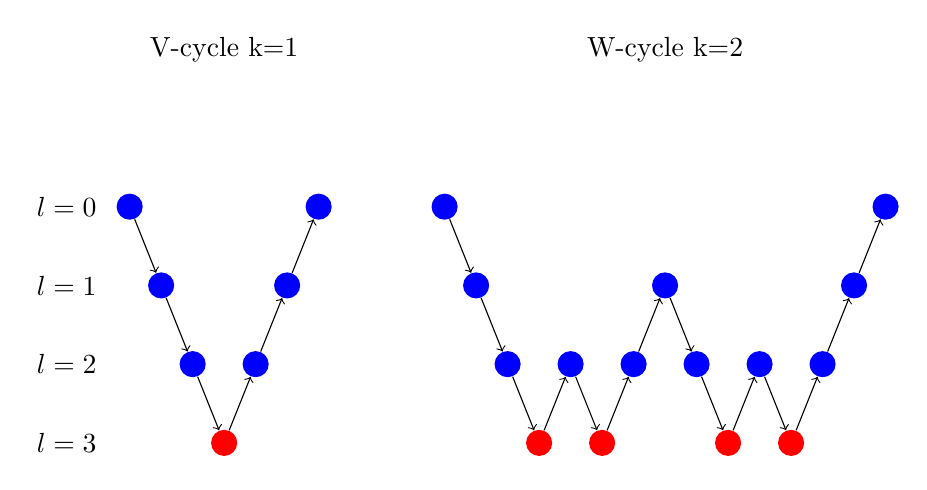
\begin{tikzpicture}
  
\begin{scope}[xscale=2/5]

  \node (sh) at (-5,3) { $l=0$ };
  \node (shh) at (-5,2) { $l=1$ };
  \node (shhh) at (-5,1) { $l=2$ };
  \node (shhhh) at (-5,0) { $l=3$};
  
  \node (title) at (0,5) { V-cycle k=1};
  \node (title2) at (14,5) {W-cycle k=2};

    \node[circle,fill=blue] (a) at (-3,3) { };
    \node[circle,fill=blue] (b) at (-2,2) {};
    \node[circle,fill=blue] (c) at (-1,1) {};
    \node[circle,fill=red] (d) at (0,0) {};
    \node[circle,fill=blue] (e) at (1,1) {};
    \node[circle,fill=blue] (f) at (2,2) {};
    \node[circle,fill=blue] (g) at (3,3) {};
    
    \draw[->] (a) -- (b);
    \draw[->] (b) -- (c);
    \draw[->] (c) -- (d);
    \draw[->] (d) -- (e);
    \draw[->] (e) -- (f);
    \draw[->] (f) -- (g);
    
    \node[circle,fill=blue] (aa) at (7,3) { };
    \node[circle,fill=blue] (ab) at (8,2) {};
    \node[circle,fill=blue] (ac) at (9,1) {};
    \node[circle,fill=red] (ad) at (10,0) {};
    \node[circle,fill=blue] (ae) at (11,1) {};
    \node[circle,fill=red] (af) at (12,0) {};
    \node[circle,fill=blue] (ag) at (13,1) {};
    \node[circle,fill=blue] (ah) at (14,2) {};
    \node[circle,fill=blue] (ai) at (15,1) {};
    \node[circle,fill=red] (aj) at (16,0) {};
    \node[circle,fill=blue] (ak) at (17,1) {};
    \node[circle,fill=red] (al) at (18,0) {};
    \node[circle,fill=blue] (am) at (19,1) {};
    \node[circle,fill=blue] (an) at (20,2) {};
    \node[circle,fill=blue] (ao) at (21,3) {};
    
    \draw[->] (aa) -- (ab);
    \draw[->] (ab) -- (ac);
    \draw[->] (ac) -- (ad);
    \draw[->] (ad) -- (ae);
    \draw[->] (ae) -- (af);
    \draw[->] (af) -- (ag);
    \draw[->] (ag) -- (ah);
    \draw[->] (ah) -- (ai);
    \draw[->] (ai) -- (aj);
    \draw[->] (aj) -- (ak);
    \draw[->] (ak) -- (al);
    \draw[->] (al) -- (am);
    \draw[->] (am) -- (an);
    \draw[->] (an) -- (ao);
    \end{scope}
    
 \end{tikzpicture}}
 \caption{V-cycle and W-cycle on 4-level grid.}
 \label{fig.cycles}
\end{figure}

A strategy will be composed of a type of cycle (V or W) and a number of relaxation steps $\alpha$. The default implementation of BomerAMG does not allow to have different values
for $\alpha_1,\alpha_2,\dots$ so we set them all to this value $\alpha$. We consider a total of 8 different stragies represented in Table~\ref{table.strat1}.
To compare the different strategies using the BoomerAMG algorithm, we run the algorithm on a predefined matrix of size $512000 \times 512000$ for every
value of maximum number of iterations (i.e. number of cycles) from 1 to 100 and with a required tolerance of $0$ (meaning
that the algorithm will stop when the result is exact or the maximum number of iterations is reached). We measure for each experiment the final relative residual norm and the execution time. Each experiment is run 10 times to have an accurate average execution time.
The results are presented on Figure~\ref{fig.first_tests}.

\begin{table}

\begin{center}
 \begin{tabular}{|c|c|c|c|c|c|c|c|c|}
   \hline
   Type of cycle & V & V & V & V & W & W & W & W \\
   \hline
   $\alpha$ & 1 & 2 & 3 & 10 & 1 & 2 & 3 & 10 \\
   \hline
 \end{tabular}
\end{center}
 \caption{8 strategies.}
 \label{table.strat1}

\end{table}


\begin{figure}
  \includegraphics[width=0.49\linewidth]{figs/convergence_1.pdf}
  \includegraphics[width=0.49\linewidth]{figs/time_convergence.pdf}
  \caption{Execution time and final residual norm of the 8 strategies per iteration (left) and convergence time as a function of the tolerance (right).}
  \label{fig.first_tests}
\end{figure}

What we can observe is that, as expected, increasing the number of relaxation steps or complexifying the cycle increases the overall time to do one cycle. However, it converges in less iterations.
We see on the right figure that actually, for a given precision, the simple V-cycle with only 1 relaxation at each step is the fastest way to reach it, followed closely by the W-cycle with $\alpha=1$.\\
The conclusion is that relaxation steps seem to be too costly for the accuracy they grant. It is better to increase the complexity of the cycle or do more cycles, thus more moves in the grid, than doing more relaxation steps. This at least proves
that multi-grid is a good alternative to classic iterative methods.


\subsection{Improving the baseline}

\subsubsection{Symmetric strategies}
Following these results, we can wonder how to improve the efficiency of the simple V-cycle with 1 relaxation step.
The first step is to analyze the time spent in the different parts of a cycle. All the different matrices $A$ for each level are computed in a setup phase so we do not need to analyze these computation times. We only focus on measuring these two different computations: (i) the time spent doing a relaxation at each level and (ii) the time spent computing the next linear system
(when going down in the grid), i.e. restricting the solution to a coarser grid, which is a sparse matrix-vector computation or the time spent interpolating the error term (when going up in the grid) which is another sparse matrix-vector computation. The values where measured for a problem (an unstructured domain with some anisotropy, denoted by Unstructed-Anisotropy) of size 512000 with a 8-level grid and are presented
in Table~\ref{table.measures}, along with some information on the matrix used at the corresponding level.

\begin{table}
  \resizebox{\linewidth}{!}{
 \begin{tabular}{|c|c|c|c|c|c|c|}
 \hline
 Level & Matrix size & Non-zero & Relax (down) & Relax (up) & Matvec (down) & Matvec (up) \\
 \hline
  1 & 512,000 & 4,042,520 & 20 ms & 20 ms & 15 ms & -\\
 \hline
  2 & 256,000 & 6,475,239 & 20 ms & 25 ms & 12 ms & 4 ms\\
 \hline
  3 & 58,893 & 2,000,513 & 8 ms & 8 ms & 3 ms & 2 ms\\
 \hline
  4 & 14,285 & 788,509 & 2 ms & 2 ms & 1 ms & 0.7 ms\\
 \hline
  5 & 4,238 & 386,333 & 1 ms & 1 ms & 0.5 ms & 0.2 ms\\
 \hline
  6 & 609 & 53,493 & 0 ms & 0 ms & 0 ms & 0 ms\\
 \hline
  7 & 69 & 2,873 & 0 ms & 0 ms & 0 ms & 0 ms\\
 \hline
  8 & 2 & 4 & 0 ms & - & - & 0 ms\\
 \hline
 \end{tabular}
 }
 \caption{Approximate times spent in the different parts of a V-cycle with $\alpha=1$.}
 \label{table.measures}
\end{table}
 In practice, we notice that the number of non-zero entries in the input matrix is correlated to the average time of a relaxation at a given level. Most importantly, in this example we see that, overall,
 the relaxation represents $\approx66\%$ of the total cost of a V-cycle (while the matrix-vector multiplications are only $\approx30\%$) and that the two first levels are from far the most expensive ones.
 With this information, there are two ideas: (i) adding more relaxations in the last levels because it is almost free or (ii) removing some relaxations in the first levels to reduce the computational cost.
 
 The following 4 strategies were then tested on this same matrix.
  \begin{itemize}
   \item \emph{Fast} : no relaxation at level 2.
   \item \emph{Fast4} : no relaxation at level 3.
   \item \emph{Fast2} : 10 relaxations at level $L-2$.
   \item \emph{Fast3} : 2 relaxations at levels $L-2,L-4,\dots,3$.
  \end{itemize}
  The strategy \emph{Fast} aims at reducing the cost of the cycle by removing the penultimate relaxation (hoping the accuracy lost at this point will be compensated by the relaxation at level 0) which is very costly.
  The strategy \emph{Fast4} is a softer version of \emph{Fast} where the relaxation at level 3 is removed, reaching less improvement of the overall execution time but being more easily compensated by the two relaxations at level 1 and 2.\\
  The strategy \emph{Fast2} executes a lot of relaxations at level $L-2$, because it should not increase by much the execution time of the V-cycle. Why choose $L-2$ level instead of $L$ or $L-1$?
  This because the relaxation at level $L$ is actually a direct solve. Thus, the error term is almost exact at level $L-1$, because the only source of error
  comes from the interpolation of $e^L$ (which is exact) into $e^{L-1}$. This is why, we might expect better results by adding relaxations at level $L-2$.
  The last strategy \emph{Fast3}, pushes this idea one step further. If we assume that doing more than one relaxation gets a really accurate error estimation at level $l$, then
  at level $l-1$ we do not need to correct a lot by doing more relaxations. However at level $l-2$ we have been through 2 interpolations since last good estimation of the error vector, hence increasing the number of relaxations again.
  As we still want not to increase the execution time a lot we stop this recursion for the first levels as they are the two most costly relaxations.
  
  \begin{figure}
  \includegraphics[width=0.49\linewidth]{figs/convergence_fast_small.pdf}
   \includegraphics[width=0.49\linewidth]{figs/time_convergence_fast_small.pdf}
   \caption{Execution time and final residual norm for the 4 new strategies on a small matrix.}
   \label{fig.newstrat_small}
  \end{figure}

  In Figure~\ref{fig.newstrat_small}, we present the results of these 4 strategies on a smaller matrix of initial size 64,000 with only a 6-level grid.
  The first thing to observe is that removing the relaxation at level 1 does not provide any benefit. It sure saves time during a cycle but the accuracy loss is tremendous.
  The other thing to notice is that adding a lot of relaxations in the last levels increases by a little the execution time while being useless on the accuracy side. This is why \emph{Fast2} and  \emph{Fast3} are not really efficient.
  
  More tests were performed on the original $512,000\times 512,000$ matrix and are presented in Figure~\ref{fig.newstrat}. We find again that the original V cycle seems to be the best as \emph{Fast3} converges in slightly less cycles, but this strategy is clearly too expensive with a bigger matrix so overall it is not as efficient as the baseline. Only the strategy \emph{Fast4} seems to be more or less equivalent to the original V cycle as it reduces a bit the cost of a cycle but the convergence rate per cycle is also slightly smaller. We also confirm that \emph{Fast} takes a lot more time to reach the maximum accuracy than any of the other strategies.
  
  \begin{figure}
  \includegraphics[width=0.49\linewidth]{figs/convergence_fast.pdf}
   \includegraphics[width=0.49\linewidth]{figs/time_convergence_fast.pdf}
   \caption{Execution time and final residual norm for the 4 new strategies on the bigger matrix.}
   \label{fig.newstrat}
  \end{figure}
  
\subsubsection{An asymmetric strategy}
\label{sec.assymetric}
  We observe no big improvement compared to the original V-cycle with 1 relaxation at each level with the previous strategies.
  Their common point is that they all do the same number of relaxations when going down or up in the cycle. However, the main idea of the multi-grid algorithm is totally asymmetric: the relaxations before
going to a coarser level is there to compute a first approximate solution to the current system while the relaxations before going back to a finer level are here to refine the error term.
  We first compute an approximation at a given level $l$, then we use the level $l+1$ to compute an approximate error term $e^l$ and finally we redo some relaxation to refine the solution. The two relaxations do not have the same goal.
  What if we could ensure that any value of the error vectors will be less than $\epsilon$ from the exact value just by doing a relaxation step? We would not need to do a relaxation
  before computing the approximate error term using the next levels in the grid but compute directly the error term when we go back up in the cycle. From that idea we define a new asymmetric strategy: we use a V-cycle with $\alpha_1 = 0$ and $\alpha_2 = 1$. In other words
  we do one relaxation at each level only when we are going up in the cycle. We call this strategy \emph{Up}.
  
  We run \emph{Up} and \emph{Fast4}, as long as the classical V-cycle, on the same matrix of size 512,000 and also on
  other applications (3D laplace with a 9-pt stencil, 3D laplace with a 27-point stencil, and another 3D partial derivative equation with Dirichlet boundary conditions) with the same size of matrix.
  
  All results are presented in Figure~\ref{fig.up_comparison}.
  
  \begin{figure}
   \subfloat[\textsc{Unstructured-Anisotropy}]{\includegraphics[width=0.49\linewidth]{figs/time_convergence_up_1.pdf}}
   \subfloat[\textsc{3DLaplace-9pt}]{\includegraphics[width=0.49\linewidth]{figs/time_convergence_up_2.pdf}}\\
   \subfloat[\textsc{3DLaplace-27pt}]{\includegraphics[width=0.49\linewidth]{figs/time_convergence_up_3.pdf}}
   \subfloat[\textsc{PDE-Dirichlet}]{\includegraphics[width=0.49\linewidth]{figs/time_convergence_up_4.pdf}}
   \caption{Comparison of original algorithm with \emph{Fast4} and \emph{Up} strategies.}
   \label{fig.up_comparison}
  \end{figure}

   At this point, we see that it is not worth considering the \emph{Fast4} strategy anymore. However, \emph{Up} seems to be
   quite efficient since it improves by $12\%$,$7\%$,$20\%$ and $22\%$ (for \textsc{Unstructured-Anisotropy}, \textsc{3DLaplace-9pt}, \textsc{3DLaplace-27pt} and \textsc{PDE-Dirichlet} respectively) the average time needed to reach
   a $10^{-i}$ precision.
   However all these runs are sequential and does not guarantee the viability of the \emph{Up} strategy when the algorithm is parallelized.
   More tests were performed on MinoTauro with bigger matrices and different processor topologies. The total size of the matrix is set to either
   5,832,000 or 13,824,000, while the topology will be composed of either 27 (3x3x3), 36 (6x6x1) or 64 (4x4x4) processors, where each processor holds 1 MPI process and there is only 1 OpenMP thread per process.
   The problems tested were \textsc{3DLaplace-9pt} and \textsc{3DLaplace-27pt}.
   For these 6 possible combinations, we observe an averaged improvement of 18.4\% (ranging from 16.0\% to 28.3\%) for \textsc{3DLaplace-9pt} and 20.5\% (ranging from 16.2\% to 25.0\%) for \textsc{3DLaplace-27pt}. It seems that \emph{Up} outperforms
   even more the classical V-cycle when the problem size increases, but seems to cap at around 25\% improvement. Figure~\ref{fig.mtup} presents the results for the matrix size 13,824,000 and \textsc{3DLaplace-27pt}, for the 3 different processor topologies. We have similar figures
   for the other scenarios.
   
   \begin{figure*}[t]
    \subfloat[3x3x3]{\includegraphics[width=0.33\linewidth]{figs/mt_27.pdf}}
    \subfloat[4x4x4]{\includegraphics[width=0.33\linewidth]{figs/mt_64.pdf}}
    \subfloat[6x6x1]{\includegraphics[width=0.33\linewidth]{figs/mt_36.pdf}}
    \caption{Comparison of original algorithm with \emph{Up} strategy for \textsc{3DLaplace-27pt} on a 240x240x240 grid.}
    \label{fig.mtup}
   \end{figure*}


\section{Investigate Time-Accuracy trade-offs}
\label{sec:accuracy}

   \subsection{A new version of multi-grid algorithm}
   If we look at the previous section, we see that at some point, even if we increase the number of cycles we do, we reach a lower bound (which depends on the topology and the problem considered) on the accuracy we can achieve (for example on Figure~\ref{fig.first_test}, it is around $10^{-15}$). This bound comes from the internal limitations of the \texttt{double} type.
   Indeed, a double uses 8 bytes (52 bits for the mantissa, 11 for the exponent and 1 bit for the sign). This representation does not allow a full description of all rational numbers (for example between $2^{52}$ and $2^{53}$ only integers can be represented).
   If we increase the number of bits of the mantissa or the exponent we can describe more and more numbers. In the other way, if we reduce it, we lose accuracy for numbers that are not representable. Considering our algorithm, what if we only want
   a precision of only $10^{-3}$ ? We don't need the 64 bits of a \texttt{double}, to reach it, a smaller number is enough. The advantage of using less bits for the floating point numbers is a faster and energy-saving computation. Thus it is important
   to study the impact of using a representation with smaller mantissa.
   
   To realize these experiments, we use two modified versions of the original algorithm. We modify the function that does the relaxation step (remember it is the costly part of the whole algorithm).
   In this function we can find different internal variables that are originally of type \texttt{double}: 5 arrays and 8 scalars. We will denote by \emph{AMG} this original algorithm. The first version, \emph{AMGfloat}, changes the type of these 13 variables from \texttt{double*} or \texttt{double}
   to \texttt{float*} or \texttt{float}. For the second version, we use the library MPFR~\cite{MPFR,MPFR_link} that introduces a type \texttt{mpfr\_t}. This type has a parameter which is the number of bits in the mantissa of the variable.
   Every computation is done exactly, meaning that it is first computed as if there was an infinite number of bits, then rounded to a number using exactly the number of bits set as parameter. We build the second version, \emph{AMGmpfr(b)}: \emph{AMGmpfr(b)} is the algorithm \emph{AMG} where the 8 scalar variables of the relaxation function are replaced
   by \texttt{mpfr\_t} variables, all using the same number of $b$ bits for the mantissa. In terms of arithmetic precision, \emph{AMG} behaves similarly to \emph{AMGmpfr(53)} and \emph{AMGfloat} to \emph{AMGmpfr(24)}. There can be small differences
   due to the rounding method used.
   
   The Figure~\ref{fig.bits_accuracy} represent the accuracy we reach using either \emph{AMGmpfr(8)}, \emph{AMGmpfr(16)}, \emph{AMGfloat}, \emph{AMGmpfr(32)} or \emph{AMGmpfr(64)}. The problem used is \textsc{Unstructured-Anisotropy}, with 2x2x2 processor topology and 20x20x20 matrix size.
   What we actually see on this figure is the threshold reachable depending on the number of bits used. However, until this threshold is reach, the accuracy obtained using any number of bits is the same. This means that, for example,
   while the accuracy of the solution is below the threshold using 32 bits, using 32 or any greater number of bits to do the computations will result in the same final accuracy. However, we expect that using only the necessary $32$ bits is 
   more efficient in terms of time, space and energy.
   
   \begin{figure} \centering
    \includegraphics[width=0.8\linewidth]{figs/bits_convergence.pdf}
    \caption{Accuracy achievable with different number of bits in mantissa. Points (except for 24 bits) were obtained only for multiples of 5 iterations, but it is enough to see the thresholds appear.}
    \label{fig.bits_accuracy}
   \end{figure}
   
   The second thing to see is that \emph{AMGfloat} behaves exactly as what we would expect from \emph{AMGmpfr(24)} (same accuracy as versions with more precision in the beginning, then it reaches a threshold between that of \emph{AMGmpfr(16)} and that of \emph{AMGmpfr(32)}) in terms of accuracy whereas more variables were changed from \texttt{double} to \texttt{float}. It does not degrade more the accuracy, only a few variables
   from the 8 scalars actually control the final precision as they are temporary variables used for intermediate computations before being plugged back into the input matrix/vector.
   That being said, we design a new algorithm that adapts the precision of the variables during the execution. It is the same algorithm as \emph{AMGmpfr(b)} except this time the precision can change between two cycles.
   We fix a threshold on the ratio between the relative residual norm at two consecutive steps to trigger the precision change.
   Figure~\ref{fig.prec_incr} presents the evolution of accuracy for the original algorithm, 3 different strategies with increasing precision and a threshold of 0.8: start at $b=16$ and do $b=b+8$, start at $b=32$
   and do $b=b+8$, and start at $b=16$ and do $b=b\times2$. We run these strategies on a 240x240x240 matrix size with a 3x3x3 topology for \textsc{3DLaplace-27pt}.
   
   \begin{figure} \centering
    \includegraphics[width=0.8\linewidth]{figs/prec_incr.pdf}
    \caption{Accuracy of adaptive algorithms compared to the original double-precision with a threshold for updating the precision of $0.8$.}
    \label{fig.prec_incr}
   \end{figure}
   
   We see some steps appear, corresponding to the lower bound on the accuracy at the current precision. Then the precision is adapted to be able to improve the overall accuracy. Even if we lose some accuracy by waiting for the ratio
   between two consecutive relative residual norm to be higher than the threshold, when the precision changes, the convergence rate is more important (for one cycle) than that of the original algorithm (i.e. the slope is bigger on the figure), which makes any of
   the 3 versions able to reach the maximum accuracy (of $4.7\times 10^{-13}$) in the same number of cycles as the original algorithm (20-21 cycles).
   
   Two questions arise at this step. How to evaluate the energy/time savings of this adaptive algorithm? Which precisions should be used to optimize these savings?\\
   The first question is not simple because the use of the MPFR library to do these accuracy experiments introduce a huge overhead in the computations (running \emph{AMGmpfr(53)} is about 20 times longer than running \emph{AMG} whereas it
   represents the final same algorithm), and this overhead is not highly influenced by the choice of the number of bits. Thus it is impossible just to measure the execution time of the algorithm using MFPR library.


\subsection{Optimal set of precisions}

In this subsection, we provide an optimal set of precisions to minimize the
total execution time, under the assumption that the time evolves linearly with
$b$ the number of precision bits: $T(b) = \alpha b + c$. \leo{This assumption
is supported by current technologies, in which double precision executions take
twice the time to complete than single precision executions. This is due to
processors having more low precision FPUs than high precision FPUs (See
previous section).}

   \begin{theorem}

       Given $b_{max}$, a maximum number of bits, $n$ the number of different
       precisions $b_1,\dots,b_n$ to use, and $T(b)=\alpha b+c$, with $\alpha$
       and $c$ two constants, the time to execute a cycle at precision $b$,
       then the execution time of our adaptive algorithm is minimized for $b_i
       = \frac{i}{n}b_{max}$.

   \end{theorem}

\begin{proof}

    From the previous experiments we can see that (i) the number of cycles
    needed to reach the lower bound for a given precision does not depend on
    the precision used during previous cycles (See Figure~\ref{fig.prec_incr}),
    i.e.  if one starts with cycles at precision $16$ bits and then switch to
    $32$ bits, you will need the same number of cycles to reach the lower bound
    with $32$ bits as if you used only cycles with $32$ bits from the beginning
    of the algorithm; and that (ii) the number of cycles needed to reach the
    lower bound is proportional to the number of bits $b$ used (See
    Figure~\ref{fig.bits_accuracy}). We then define $\textsc{MaxIter}(b)$ the
    number of cycles needed so that the ratio between the relative
    residual norms computed before and after these cycles is higher than a threshold $t$. 
    We use the two observations
    to model $\textsc{MaxIter}(b) = \lfloor kb \rfloor$ for some constant $k$.
    Then we can compute the total execution time:

    \begin{align*}
        T_{total}& = \textsc{MaxIter}(b_1)T(b_1)\\ & +  \sum\limits_{i=1}^{n-1}
        (\textsc{MaxIter}(b_{i+1})-\textsc{MaxIter}(b_i))T(b_{i+1}).
    \end{align*}

    Indeed, when we reach the number of iterations $\textsc{MaxIter}(b_i)$ we
    change from precision $b_i$ to precision $b_{i+1}$.  We can rewrite
    $T_{total}$ as

    \begin{align*}
        T_{total} &\approx k b_{1} T(b_1) + \sum\limits_{i=1}^{n-1}
        k(b_{i+1}-b_{i})T(b_{i+1})\\ & \approx k ( b_{n}T(n) +
        \sum\limits_{i=1}^{n-1} b_i ( T(b_i) - T(b_{i+1})).
    \end{align*}

    By plugging the expression of $T(b)$ into the previous equation and considering
    the maximum precision we want is $b_{max}=b_n$, we finally get:

    \begin{equation}
        T_{total}  = k\alpha\left(b_n^2 + \sum\limits_{i=1}^{n-1} (b_i^2 - b_i b_{i+1})\right) + kb_{max}c.
    \end{equation}

    Let us consider the function $f(x_1,\dots,x_n) = \sum\limits_{i=1}^n x_i^2
    - \sum\limits_{i=1}^{n-1} x_ix_{i+1}$. Finding the minimum of
    $f(x_1,\dots,x_{n-1},1)$ will give us the minimum of the execution time.

    By simple partial derivation: \[ \frac{\partial f(x_1,\dots,x_n)}{\partial
    x_i} = 2x_i - (1-\delta_{i,n})x_{i+1} - (1-\delta_{i,1})x_{i-1} \] where
    $\delta_{a,b} $ is equal to 1 if and only if $a=b$, 0 otherwise.

    This is where the boundary condition $x_n = 1$ is useful: if we do not set it
    to a number different from 0, the function is minimized for
    $x_1=\dots=x_n=0$. Applying this to our problem makes no sense, as we
    would not be doing any computation. The boundary condition represents the
    fact that we need to reach an existing precision ($b_{max}$) eventually. By
    a simple scaling, considering $1$ instead of $b_{max}$ makes computation
    easier and does not change the resolution of the the following system (up
    to a factor):

    \resizebox{0.9\linewidth}{!}{
    $\left\{
    \begin{tabular}{rcl cccccccccc cl}
    $\frac{\partial f(x_1,\dots,x_n)}{\partial x_1}$ & = & $2x_1$ & $-$ & $x_2$  &     &       & & 	 &&     &     &       & = & 0 \\
    $\frac{\partial f(x_1,\dots,x_n)}{\partial x_2}$ & = & $-x_1$ & $+$ & $2x_2$ & $-$ & $x_3$ & & 	 &&     &     &       & = & 0 \\
    & \vdots &&&&&&&&&&&&&\\
    $\frac{\partial f(x_1,\dots,x_{n})}{\partial x_{n-1}}$ & = &        &     &        &     &       & & $-x_{n-2}$ & $+$ & $2x_{n-1}$ & $-$ & $x_n$ & = & 0 \\
    $x_n$ & = & 1 &&&&&&&&&&&&\\
    \end{tabular} \right.$
    }

    Solving this system of equations is equivalent to solving the linear system $Ax=b$ where
    \[ A =
    \begin{bmatrix}
    2       & -1 &  &  &  \\
    -1       & 2 & -1 &  &  \\
    & \ddots & \ddots & \ddots & \\
    & & -1 & 2 & -1 \\
           &  &  & -1 & 2
    \end{bmatrix}
    \textup{ and } b = \begin{bmatrix} 0 \\ \vdots \\ 0 \\ 1 \end{bmatrix} \]

    This system has a unique solution which is $\begin{bmatrix} \frac{1}{n} & \dots
    & \frac{n-1}{n} \end{bmatrix}$.  The minimum of $f(x_1,\dots,x_n)$ with
    boundary condition $x_n=1$ is thus reached for $x_i = \frac{i}{n}$.  It
    is, when multiplied by $b_{max}$, the solution that minimizes our total
    execution time.

\end{proof}

   This proof holds only if the execution time evolves linearly with $b$, but
   \textit{we could also apply it to minimize the energy consumption} assuming
   that the energy consumption of one cycle increases linearly with $b$. In the
   next section we investigate whether this assumption holds.



\subsection{Evaluation}
   
   In order to estimate the cost of our algorithm, we want to model the time of an iteration at precision $b$. We model an iteration by the following formula: $an^3b^\alpha+c$, where $a,c$ and $\alpha$ are constants,
   $n$ is the size of the problem and $b$ the number of bits. Indeed, we expect the time to be proportional to the cube of the problem size as we deal with 3D problems, and the parameter $\alpha$ will characterize how the time evolves when we double the number of bits: if $\alpha = 1$, then multiplying by two the number of bits will multiply by two the cost of an iteration. Maybe the reality should be described by a more complicated polynomial in $b$, but we want to keep the model simple enough and see if the data can fit it.
   

%    To provide numerical values for $a$,$\alpha$ and $\beta$, we measured the execution times of different scenarios. Each scenario computes 50 iterations on a 64x64x64 matrix, on different processor topologies, and using
%    either only single-precision floating point variables or only double-precision floating point variables. We denote by $x_{b,n}$ the empirical value obtained using $b$ bits and $n$ processors. Results are reported in Table~\ref{table.time_measure1}.
%    \iffalse
%    P1x1x1, 10 iterations, average on ten runs\\
%    \begin{tabular}{|l|c|c|c|c|}
%    \hline
%     \multirow{2}{*}{Experiment} & \multicolumn{2}{c|}{Single-Precision} & \multicolumn{2}{c|}{Double-precision} \\
%     \cline{2-5}
%     & Solve (s) & Cycle (ms) & Solve (s) & Cycle (ms) \\
%     \hline
%     (1) 40x40x40 & 1.308 & 12 & 1.543 & 14\\
%     \hline
%     (1) 80x80x80 & 10.794 & 100 & 13.033 & 121.5\\
%     \hline
%     (2) 20x20x20 & 0.1316 & 1.1 & 0.1411 & 1.2 \\
%     \hline
%     (2) 40x40x40 & 1.026 & 9.5 & 1.195 & 11 \\
%     \hline
%     (2) 80x80x80 & 8.068 & 74 & 9.595 & 88 \\
%     \hline
%      (3) 20x20x20 & 0.170 & 1.4 & 0.179 & 1.5 \\
%     \hline
%      (3) 40x40x40 & 1.396 & 11.5 & 1.646 & 13.7 \\
%     \hline
%      (3) 80x80x80 & 10.644 & 89 & 12.572 & 106 \\
%     \hline
%      (4) 20x20x20 & 0.1405 & 1.2 & 0.149 & 1.3 \\
%     \hline
%      (4) 40x40x40 & 1.192 & 11 & 1.402 & 15\\
%     \hline
%      (4) 80x80x80 & 10.258 & 96 & 12.125 & 114 \\
%     \hline
%    \end{tabular}
%    
%    Jacobi\begin{tabular}{|l|c|c|c|c|}
%    \hline
%     \multirow{2}{*}{Experiment} & \multicolumn{2}{c|}{Single-Precision} & \multicolumn{2}{c|}{Double-precision} \\
%     \cline{2-5}
%     & Solve (s) & Cycle (ms) & Solve (s) & Cycle (ms) \\
%     \hline
%     (1) 40x40x40 & 0.0868 & 7.8 & 0.09577 & 8.4\\
%     \hline
%     (1) 80x80x80 & 0.709 & 63 & 0.8757 & 73\\
%     \hline
%     (2) 20x20x20 & 0.00945 & 0.8 & 0.00991 & 0.9 \\
%     \hline
%     (2) 40x40x40 & 0.0755 & 6.5 & 0.0815 & 7.2 \\
%     \hline
%     (2) 80x80x80 & 0.581 & 51 & 0.648 & 57 \\
%     \hline
%      (3) 20x20x20 & 0.0121 & 0.95 & 0.0126 & 1.0 \\
%     \hline
%      (3) 40x40x40 & 0.0990 & 7.8 & 0.105 & 8.2 \\
%     \hline
%      (3) 80x80x80 & 0.759 & 60 & 0.878 & 75 \\
%     \hline
%      (4) 20x20x20 & 0.0104 & 0.92 & 0.0106 & 1.0 \\
%     \hline
%      (4) 40x40x40 & 0.0842 & 7.6 & 0.0972 & 8.8\\
%     \hline
%      (4) 80x80x80 & 0.720 & 64.5 & 0.810 & 75.5 \\
%     \hline
%    \end{tabular}
% \fi
%   \begin{table}
%   \begin{center}
%    \begin{tabular}{|l|c|c|c|c|}
%    \hline
%     \multirow{2}{*}{Experiment} & \multicolumn{2}{c|}{Single-Precision} & \multicolumn{2}{c|}{Double-precision} \\
%     \cline{2-5}
%     & Solve (s) & Cycle (ms) & Solve (s) & Cycle (ms) \\
%     \hline
%     1x1x1 & 2.1853 & 70-80 & 2.6874 & 90 \\
%     \hline
%     2x1x1 & 1.3912 & 40-50 & 1.6476 & 50-60\\
%     \hline
%     2x2x1 & 0.8544 & 30-40 & 0.9943 & 40-50 \\
%     \hline
%     2x2x2 & 0.5393 & 10-20 & 0.6935 & 10-20 \\
%     \hline
%     4x2x2 & 0.3255 & 0-10 & 0.3802 & 10 \\
%     \hline
%     4x4x2 & 0.2542 & 0-10 & 0.2815 & 0-10 \\
%     \hline
%     4x4x4 & 0.3171 & 0-10 & 0.362 & 0-10 \\
%     \hline
%    \end{tabular}
%    \end{center}
%    \caption{Execution times of AMG solver using either single or double precision.}
%    \label{table.time_measure1}
%  \end{table}
%    
%    The first thing to notice is that increasing the number of processors decreases the execution times, except when going from 32 to 64. This is because the matrix becomes very small and the communication costs become too important.
%    We won't use theses two values for what follows.
%    We now need to find values of $a,\alpha$ and $\beta$ that fit our measures.\\
%    We will change from $a$ to a new $a'$ by setting $f(b,n) = \frac{a'}{n^\beta} \left(\frac{b}{32}\right)^\alpha$. Now if we look only at the 6 points for $b=32$, we just have $f(32,n) = \frac{a'}{n^\beta}$, which does not
%    depend on $\alpha$. To fit our data, we evaluate the least squares sum, that is to say $\sum\limits_{i=0}^5 (f(32,2^i)-x_{32,2^i})^2$. We want it to be minimized, so choosing the best $a$ is done by choosing
%    $\frac{x_{32,1}*1^\beta + \dots + x_{32,32}*32^\beta}{6}$. Then the minimal sum is obtained for $\beta \approx 0.634$, giving $a' \approx 2.099$.\\
%    Finally, we evaluate the least squares sum using all the 12 values to find the value of $\alpha$. The result found in this case is $\alpha \approx 0.3157$. To come back to the original formula we just have to divide $a'$ by $32^\alpha$, and we obtain
%    the final following formula:
%    \[ f(b,n) \approx \frac{0.703}{n^{0.634}} b^{0.3157}. \]
%    
%    Now that we modeled how time increases when $b$ incrases, we can evaluate different strategies that use.
%    
%    \iffalse
%    (1) 64x64x64, 50 iterations, averaged on 100 runs (Jacobi)\\
%    \begin{tabular}{|l|c|c|c|c|}
%    \hline
%     \multirow{2}{*}{Experiment} & \multicolumn{2}{c|}{Single-Precision} & \multicolumn{2}{c|}{Double-precision} \\
%     \cline{2-5}
%     & Solve (s) & Cycle (ms) & Solve (s) & Cycle (ms) \\
%     \hline
%     1x1x1 & 1.3731 & 40-50 & 1.6986 & 50-60\\
%     \hline
%     2x1x1 & 0.9028 & 30 & 1.1481 & 40-60\\
%     \hline
%     2x2x1 & 0.593 & 20 & 0.7015 & 30-40 \\
%     \hline
%     2x2x2 & 0.3762 & 10 & 0.5316 & 10-20 \\
%     \hline
%     4x2x2 & 0.2447 & 0-10 & 0.2681 & 0-10 \\
%     \hline
%     4x4x2 & 0.2032 & 0-10 & 0.2362 & 0-10 \\
%     \hline
%     4x4x4 & 0.3086 & 0-10 & 0.3477 & 0-10 \\
%     \hline
%    \end{tabular}
%   \fi
%   
%     \includegraphics[width=\textwidth]{figs/3157_3.pdf}\\
%     \includegraphics[width=\textwidth]{figs/3157_5.pdf}\\
%     \includegraphics[width=\textwidth]{figs/3157_7.pdf}\\
%     \includegraphics[width=\textwidth]{figs/3157_10.pdf}\\
%     \includegraphics[width=\textwidth]{figs/3157_15.pdf}

   To provide numerical values for $a,c$ and most importantly $\alpha$, we measure the execution times of different scenarios. Each scenario computes 50 iterations on matrices with different sizes, and using
   either only single-precision floating point variables or only double-precision floating point variables. We denote by $x_{b,n}$ the empirical value obtained using $b$ bits and a problem of size $n$ (i.e. the matrix
   considered will be of size $n^3 \times n^3$ as we consider 3D problems). %Results are reported in Table~\ref{table.time_measure1}.
   
   Then, using Python's lmfit package, we interpolate the data to find good values for $a,c$ and $\alpha$. We are able to estimate different values of $\alpha$, all between 0.20 and 0.32, using 3
   different applications, 2 types of cycles (the classic V-cycle and the \emph{Up} strategy) and 2 types of relaxation method (weighted Jacobi and an hybrid method).
   With these values of $\alpha$, we can estimate the cost of our algorithm in units of time by $\left(\frac{b}{53}\right)^\alpha$ for a cycle (1 unit = 1 V-cycle at double-precision) with $b$ the number of significant
   bits (i.e. the number of bits in the mantissa plus one, as one bit is always assumed in standard floating point representation). Then using the MPFR library we can create different
   scenarios that set the number of bits used at each cycle in a different way. We define all these scenarios by the first precision ($b$ in the manstissa)) used and how to update it ($delta$ bits added in the mantissa when the threshold is reached for a given precision).
   Strategies are denoted as $b\_delta$.
   This can be either an addition or a multiplication. In particular, we provide a scenario where the available precisions are 11, 24 and 53 (represented by a starting precision of 11 and a multiplicator of 2.24). This
   corresponds to the case where half-precision, single-precision and double-precision floating points are available, as it is the case on GPUs.
   
   \begin{figure*}
    \includegraphics[width=0.33\linewidth]{figs/cost_3.pdf}
    \includegraphics[width=0.33\linewidth]{figs/cost_7.pdf}
    \includegraphics[width=0.33\linewidth]{figs/cost_15.pdf}
    \caption{Cost of the MG solver considering several different dynamic accuracy scenarios to reach different error degrees in the output: $10^{-3}$ on the left, $10^{-7}$ in the middle and $10^{-15}$ on the right.}
    \label{fig.estimation1}
   \end{figure*}
   %\begin{figure}
   % \includegraphics[width=\linewidth]{figs/cost_5.pdf}
   % \caption{}
   % \label{fig.estimation2}
   %\end{figure}
   %\begin{figure}
   % \includegraphics[width=\linewidth]{figs/cost_7.pdf}
   % \caption{}
   % \label{fig.estimation3}
   %\end{figure}
   %\begin{figure}
   % \includegraphics[width=\linewidth]{figs/cost_10.pdf}
   % \caption{}
   % \label{fig.estimation4}
   %\end{figure}
   %\begin{figure}
   % \includegraphics[width=\linewidth]{figs/cost_15.pdf}
   % \caption{}
   % \label{fig.estimation5}
   %\end{figure}
   
   Figure~\ref{fig.estimation1} represents the cost of the MG solver, for these different scenarios, to reach different accuracy degrees in the output ($10^{-3}$ on the left, $10^{-7}$ in the middle and $10^{-15}$ on the right) using
   a value for the $\alpha$ parameter of 0.3. We can see that the strategy that increases by only 1 the number of mantissa bits (labelled \texttt{8\_1}) takes more time than the original algorithm (labelled \texttt{53\_0}) for the 5 different accuracies presented. This is because, in the previous experiments we saw
   there is usually the same number of cycles in all our strategies (see Figure~\ref{fig.prec_incr}). Here, the convergence rate is limited by the slowly increasing number of precision bits: by adding one bit we can divide by at most 2 the 
   accuracy on the residual norm while the original algorithm can divide by more than that in one cycle if it is not limited by the bitwidth of the variables.
   If we focus on a case starting with half precision, then going to single and finally to double precision (labelled \texttt{11\_x2.24}), we can see that, compared to the original algorithm (which uses only double-precision), we improve by 35\% the time to reach 
   accuracy $10^{-3}$ (see Figure~\ref{fig.estimation1}). If one adapts the algorithm to use only single-precision variables (labelled \texttt{24\_0}) as it would be sufficient to reach this accuracy, we would still reduce the time by 17\% (still Figure~\ref{fig.estimation1}). Then the improvement slowly decreases when increasing the accuracy to reach 10\% (for $10^{-15}$ on Figure~\ref{fig.estimation1}).
   
   \subsection{Summary of results}
   
   Finally, we want to see how changing the precisions during the algorithm also improves the execution time when we use the \emph{Up} strategy, defined in section~\ref{sec.assymetric}, compared to using the original algorithm (single or double precision).
   The table~\ref{table.results1} presents the different estimated times (in time units where 1 time unit is a V-cycle at double precision)
   for all 4 different algorithms: V-cycle (double precision), \emph{Up}-cycle (double precision), V-cycle (adaptive precisions 11-24-53), \emph{Up}-cycle (adaptive precisions 11-24-53) for Problem 1, using a hybrid relaxation method.
   We also present the improvement of the best method (i.e. \emph{Up}-cycle with different precisions) compared to the original algorithm (in double-precision and in single-precision when possible).
  
  \begin{table*}[t]
   \begin{center}
  \resizebox{\textwidth}{!}{
  \begin{tabular}{|c|c|c|c|c|c|c|}
    \hline
    Tolerance & Baseline (DP) & \emph{Up}-cycle (DP) & Adaptive (V-cycle) & Adaptive (\emph{Up}-cycle) & Improvement (DP) & Improvement (SP) \\
    \hline
    \hline
    1e-01 & 1.000 & 1.333 & 0.624 & 0.832 & 16.8\% & -5.5\%\\
    \hline
    1e-02 & 3.000 & 2.000 & 1.872 & 1.664 & 44.5\% & 29.7\%\\
    \hline
    1e-03 & 5.000 & 4.667 & 3.284 & 3.131 & 37.4\% & 20.6\%\\
    \hline
    1e-04 & 8.000 & 7.333 & 5.650 & 5.234 & 34.6\% & 17.0\%\\
    \hline
    1e-05 & 11.000 & 10.0 & 8.015 & 7.336 & 33.3\% & 15.4\% \\
    \hline
    1e-06 & 14.000 & 12.667 & 10.380 & 9.439 & 32.6\% & 14.5\%\\
    \hline
    1e-07 & 17.000 & 15.333 & 13.169 & 11.964 & 29.6\% & -\\
    \hline
    1e-08 & 20.000 & 18.000 & 16.169 & 14.631 & 26.8\% & -\\
    \hline
    1e-09 & 23.000 & 20.667 & 19.169 & 17.298 & 24.8\% & -\\
    \hline
    1e-10 & 26.000 & 24.000 & 22.169 & 20.631 & 20.7\% & -\\
    \hline
    1e-11 & 29.000 & 26.667 & 25.169 & 23.298 & 19.7\%& -\\
    \hline
    1e-12 & 32.000 & 29.333 & 28.169 & 25.964 & 18.9\% & -\\
    \hline
    1e-13 & 35.000 & 32.000 & 31.169 & 28.631 & 18.2\% & -\\
    \hline
    1e-14 & 38.000 & 34.667 & 34.169 & 31.298 & 17.6\% & -\\
    \hline
    1e-15 & 43.000 & 39.333 & 39.169 & 35.964 & 16.4\% & -\\
    \hline
  \end{tabular}
  }
  \end{center}
   \caption{All estimated times for Problem 1, size 40, hybrid relaxation method, on a single processor, with $\alpha = 0.3$. The column `Improvement (DP)' corresponds to
   the improvement between our adaptive algorithm using a \emph{Up}-cycle (column 5) compared to the original V-cycle with fixed double-precision (column 2). The column `Improvement (SP)' corresponds
   to the improvement between our adaptive algorithm using a \emph{Up}-cycle (column 5) compared to the original V-cycle with fixed single-precision.}
   \label{table.results1}
   \end{table*}
   
   The main result is that even to reach the maximum precision, we improve the execution time by more than 15\%. When it comes to smaller precisions, this improvement can be as high as 30\% compared to
   a single-precision algorithm and it even goes up to 45\% compared to the original double-precision version. We insist to remember that these results for the adaptive algorithm use 3 different precisions (11,24,53)
   whereas if other architectures would be available it would be possible to improve even more the execution by using more different precisions. For example, as we see on Figure~\ref{fig.estimation1}, using precisions
   4,8,12,16,\dots,48,52,53 should lead to a faster execution for reaching $10^{-15}$.


\section{Related Work}
\label{sec:related}


   
   Some approximate computing techniques at hardware level exist and could be applied in addition to our ideas. They include fast but slightly incorrect adders~\cite{Gupta:2011}, or voltage-scaling (in SRAM, reducing
   the voltage by 80\% increases the probability of an unexpected bit flip by around $10^{-5}$~\cite{Sampson:2011})
   if we are more interested in reducing the energy consumption instead of the execution time.\\
   Concerning multi-grid algorithms, the opposite of our \emph{Up} strategy has been considered in~\cite{JAMESON}: they do some actual computation when going down in the grid and then simply interpolate to retrieve the solution on the finest grid. The reason for that is that they
   address a specific problem where some perturbations need to be damped quite efficiently, which is why as soon as they perform some computation on the fine grid they need to use coarse grids even if interpolating directly introduces some errors.
   Dynamically changing the bit-width of some variables has been done in~\cite{Park:2010} but it is there applied on some part of the data as they are not involved in the same way in the algorithm,
   which is not the case in a multi-grid solver (all the evaluation points on the grid represent the continuous solution).

\section{Conclusion}
\label{sec:conclusions}

\section{Conclusion}
\label{sec:conclusions}

This paper improves the original MG algorithm by two different ways: 
The first one is to remove some relaxation steps in a V-cycle, which leads to faster cycles although requires more of them to converge.
Overall, this solution achieves up to 30\% improvement although its performance enhancements vary a lot depending on the workload,
The second way to improve the algorithm is to adapt the precisions of the floating point depending on MG's precision requirements,
We use low precisions levels during the very first MG's cycles and we increase them as the execution progresses. 
Repeating this operation until reaching the maximum available accuracy available leads to significant speedups.
We estimate the benefits of these two approaches combined on different scenarios. 
When combining half-, single- and double-precisions, we can reduce by 16.4\% and 14.5\% the execution time using double- or single-precision, respectively, during the whole execution. 

In the future we plan to explore additional ideas to reduce the execution time even more like changing the precision used in different levels of a cycle. 
%However, we think that it is not
%   useful because (1) using a greater precision in the coarse levels than in the fine levels is useless as all the computations would eventually be truncated and (2) using a smaller
%   precision in the coarse levels than in the fine levels would not affect by much the execution time as, according to the measurements done, only the first 2 or 3 levels represent more than 95\% of the relaxation cost of a cycle.
Also, we plan to estimate the impact of our techniques on the energy consumption by obtaining some measurements on real machines.
Evaluating the energy consumption using different values of the $\alpha$ parameter is also in our immediate future plans.


\bibliography{biblio}
\bibliographystyle{plain}

\end{document}
